\documentclass[tikz,border=2pt]{standalone}
\usepackage{amsmath,amssymb}
\usepackage{pgfplots}
\pgfplotsset{compat=1.18}

\begin{document}
% ||x||_∞ <= ||x||_2 <= sqrt(2) ||x||_∞ in R^2: the Euclidean unit circle sits between the
% square {||x||_∞ <= 1} and the smaller square {||x||_∞ <= 1/sqrt 2}. Equivalent norms squeeze
% each other's unit balls between two scalings.
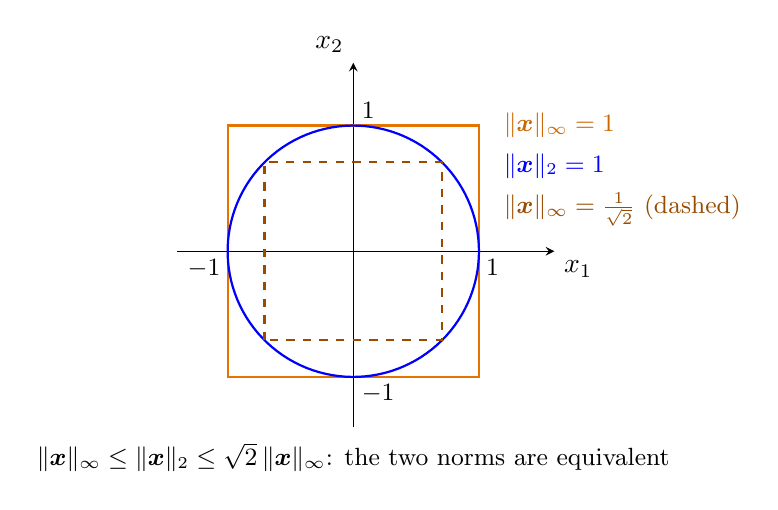
\begin{tikzpicture}
	\begin{axis}[
		axis lines=middle, axis equal image,
		xmin=-1.4, xmax=1.6, ymin=-1.4, ymax=1.5,
		xtick=\empty, ytick=\empty,
		xlabel={$x_1$}, ylabel={$x_2$},
		xlabel style={below right}, ylabel style={above left},
		samples=200, clip=false, width=7.2cm
		]
		\draw[thick, orange!90!black] (axis cs:-1,-1) rectangle (axis cs:1,1);
		\addplot[thick, blue, domain=0:360, samples=120] ({cos(x)}, {sin(x)});
		\draw[thick, orange!60!black, dashed] (axis cs:-0.7071,-0.7071) rectangle (axis cs:0.7071,0.7071);
		\node[anchor=north west, font=\small, inner sep=1.5pt] at (axis cs:1.02,-0.03) {$1$};
		\node[anchor=north east, font=\small, inner sep=1.5pt] at (axis cs:-1.02,-0.03) {$-1$};
		\node[anchor=south west, font=\small, inner sep=1.5pt] at (axis cs:0.03,1.02) {$1$};
		\node[anchor=north west, font=\small, inner sep=1.5pt] at (axis cs:0.03,-1.02) {$-1$};
		\node[orange!80!black, anchor=west, font=\small] at (axis cs:1.12,1.0) {$\|\boldsymbol{x}\|_\infty=1$};
		\node[blue, anchor=west, font=\small] at (axis cs:1.12,0.68) {$\|\boldsymbol{x}\|_2=1$};
		\node[orange!60!black, anchor=west, font=\small] at (axis cs:1.12,0.33) {$\|\boldsymbol{x}\|_\infty=\tfrac1{\sqrt2}$ (dashed)};
		\node[anchor=north, font=\small] at (axis cs:0,-1.45) {$\|\boldsymbol{x}\|_\infty\le\|\boldsymbol{x}\|_2\le\sqrt2\,\|\boldsymbol{x}\|_\infty$: the two norms are equivalent};
	\end{axis}
\end{tikzpicture}
\end{document}
